\subsection{Estimation methods}
% 3 pages
The use of estimating tasks is always relevant. Even though one does not always actively make these estimation on small project/task, one does always have some idea of how long the task will take. This knowledge is essential for planning a project because it will shed lights on how long time certain tasks will take, and allow the usage of more different planning methods.\\
Using estimation methods allowed us to be precise and thorough in our estimations, and gave us an idea of how long time each tasks takes. Based on that knowledge, we could make more precise plans to help us overcome the derailed project.

In the following we will present the methods we have used to estimate our tasks for the project. We will describe our thoughts on how we experienced the use of these methods and argue for not using certain other methods.
\subsubsection{Planning Poker}
Multiple estimation methods exists, but for this part of the project, we have chosen to use Planning Poker, also know as Scrum Poker, to estimate the remaining tasks. Planning Poker is a good practice when using Scrum, and in a sense to use the WBS/PBS paradigm (in Scrum the backlog).

Planning Poker seemed like a good choice since we all have worked with Scrum before, but not used Planning Poker, so this was a great opportunity to practice it. Also the fact that the players does not influence each other when estimating, but the game still facilitates shorts discussion is a great advantage. The fact that the `game' facilitates discussions is the reason for why we chose Planning Poker instead of the Delphi estimation method, which does not. The discussion might not always be an advantage, though. It can easily become very time consuming. We chose a non-voting, but overruling, moderator to address this potential problem, and it worked perfectly and it was an advantage multiple times.\\
We could quite quickly ignore the Analogy method since it uses comparison of similar project, which we have not done before, hence it was not an option.

\begin{figure}[H]
%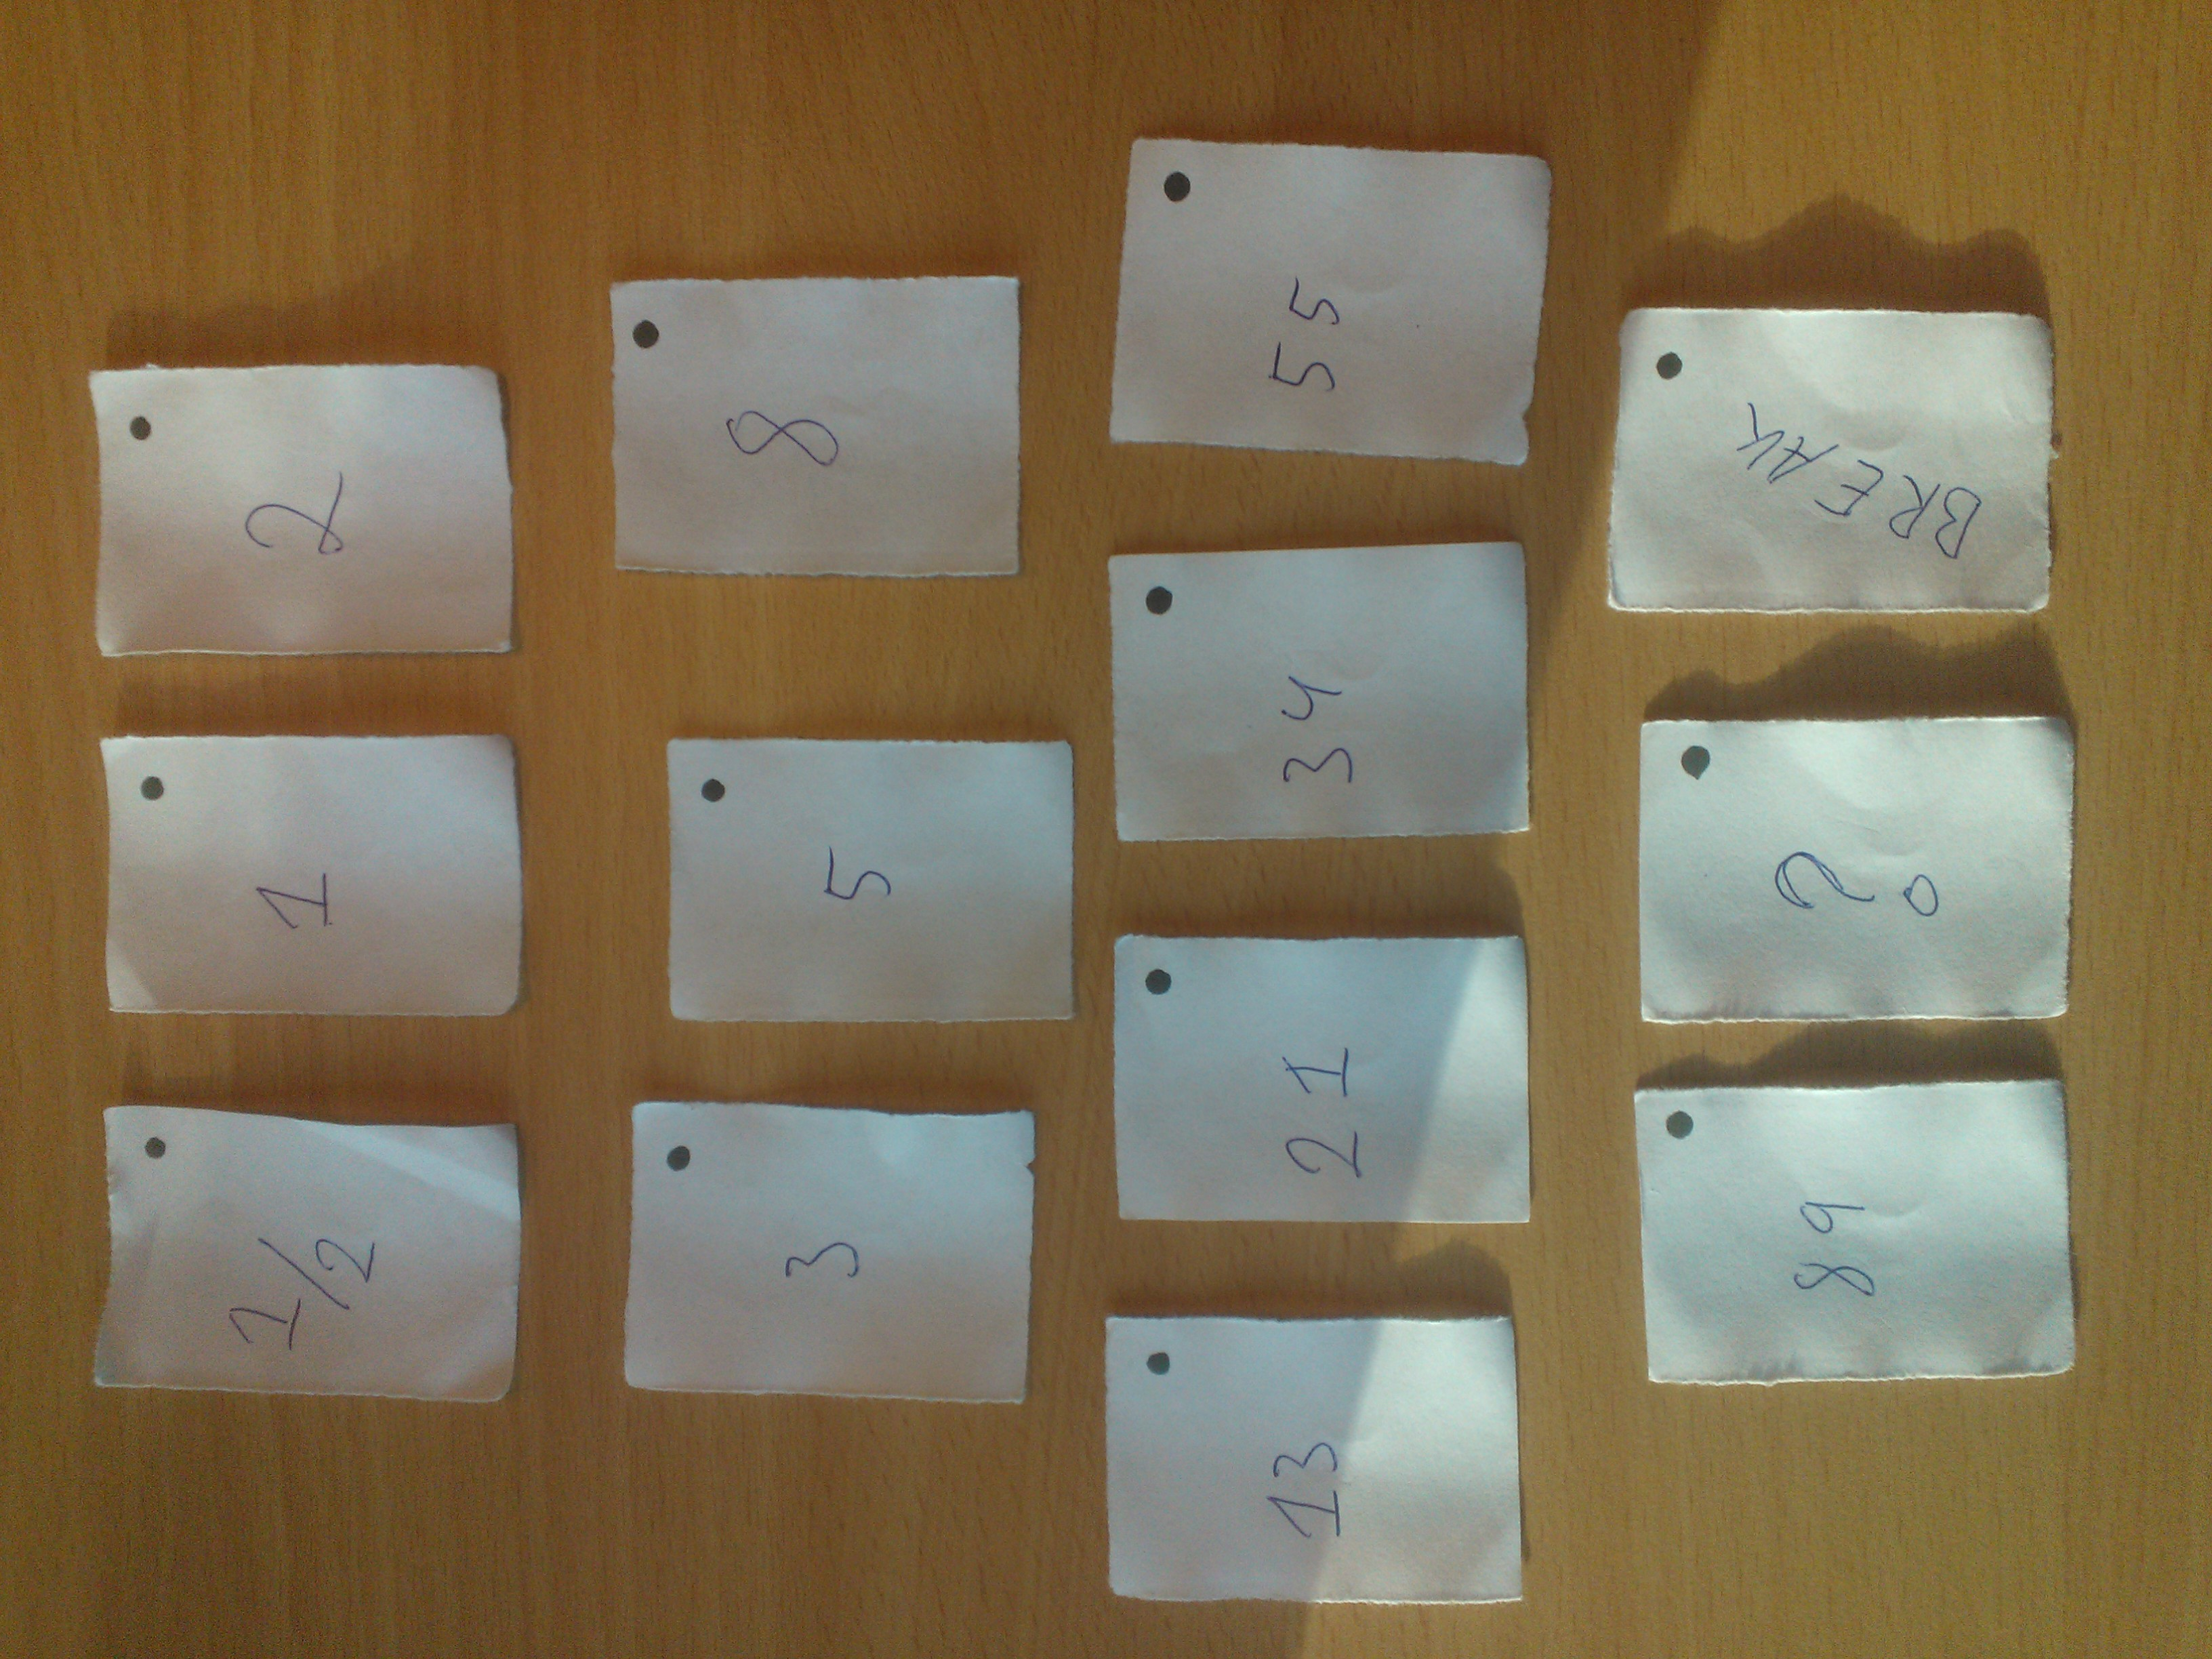
\includegraphics[width=\textwidth,natwidth=2157,natheight=1336]{illustrations/scrumPokerCards.jpg}
  \caption{Scrum poker cards}
  \label{scrumPokerCards}
\end{figure}

We made playing cards with the numbers 1/2, 1, 2, 3, 5, 8, 13, 21, 34, 55, 89, `?' and `break'. The numbers represented man hours and the question-mark represented that the `player' was unsure about the amount of work in the task, and the "break" card represented that the player needed a short break from the game.\\
We found that using Planning poker was a great advantages compared to what we previously have done. Beside the work-related advantages we also found it way more motivating than other methods, and all members of the group was included in the process. Yet, the high numbers (34, 55 and 89) was never used, as well as the `break' card. The `?' was only rarely used, and almost not considered a valid card by the team, due to the fact when playing the card the player did not participate in the discussion. Also there where the risk of only one person having a real estimation vote for the task.

\subsubsection{CoCoMo estimation}
\subsubsection{PERT estimation}